\section*{Goniometrické a cyklometrické funkce}

\textbf{Goniometrické} (též trigonometrické) funkce jsou $\sin x$, $\cos x$, $\tg x$ a $\cotg x$. Funkce k nim inverzní, $\arcsin x$, $\arccos x$, $\arctg x$ a $\arccotg x$ nazýváme \textbf{cyklometrické}.

\subsubsection*{Arkussinus}

Graf funkce $\sin x$ je na obrázku \ref{fig:sinus}. Platí $D(\sin x) = \R$ a $H(\sin x) = [-1,1]$. Nyní potřebujeme vybrat interval, na kterém je tato funkce prostá, abychom k ní mohli nalézt inverzní. Zároveň chceme pokrýt \uv{co největší obor hodnot}. Nabízí se interval $[-\pi/2, \pi/2]$. Definujeme tedy funkci \textbf{arkussinus} $\arcsin x$ předpisem \begin{align}
    D(\arcsin x) = H(\sin x) = [-1,1] \:, \quad H(\arcsin x) = [-\pi/2, \pi/2] \:, \quad \arcsin(x) = y \Longleftrightarrow x = \sin y \:.
\end{align}

\begin{figure}[H]
    \centering
    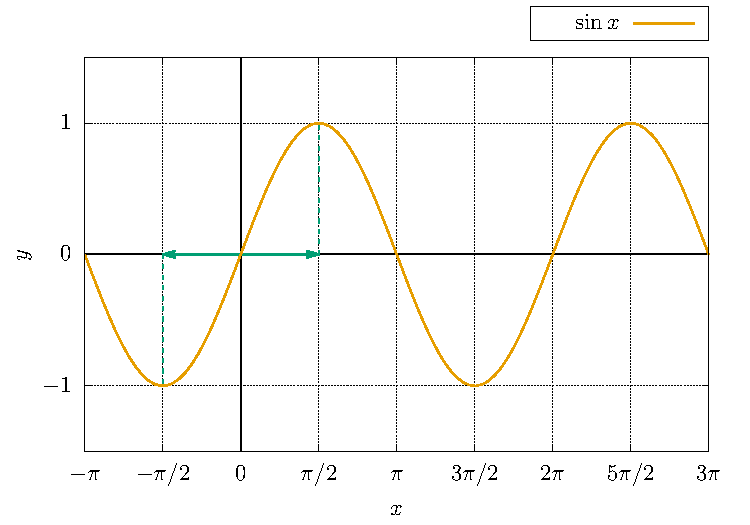
\includegraphics{Gnuplot/cv1/Figures/sinusgraf.pdf}
    \caption{Graf funkce sinus. Zeleně je vyznačen interval, kde je funkce prostá. Ten zvolíme jako obor hodnot funkce arkussinus.}
    \label{fig:sinus}
\end{figure}


\subsubsection*{Arkuskosinus}

Graf funkce $\cos x$ je na obrázku \ref{fig:kosinus}. Platí $D(\cos x) = \R$ a $H(\cos x) = [-1,1]$. Opět se chceme omezit na interval, kde je funkce prostá. Správný interval bude $[0,\pi]$. Definujeme funkci \textbf{arkuskosinus} $\arccos x$ předpisem \begin{align}
    D(\arccos x) = H(\cos x) = [-1,1] \:, \quad H(\arccos x) = [0, \pi] \:, \quad \arccos(x) = y \Longleftrightarrow x = \cos y \:.
\end{align}

\begin{figure}[H]
    \centering
    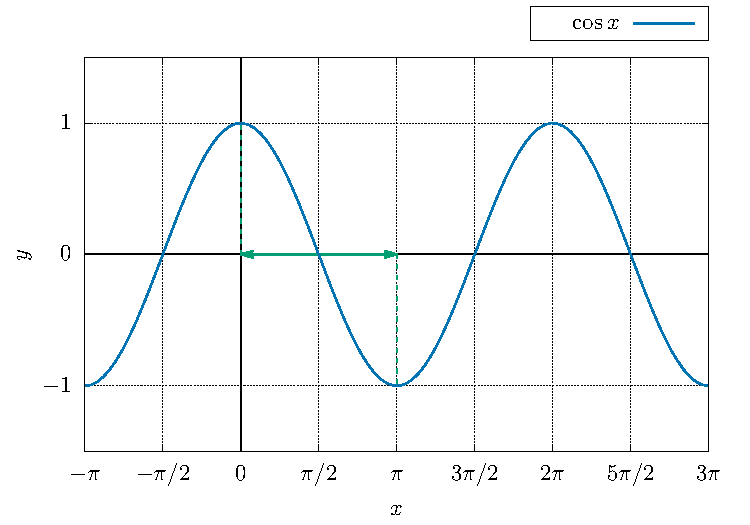
\includegraphics{Gnuplot/cv1/Figures/cosinusgraf.pdf}
    \caption{Graf funkce kosinus. Zeleně je vyznačen interval, kde je funkce prostá. Ten zvolíme jako obor hodnot funkce arkuskosinus.}
    \label{fig:kosinus}
\end{figure}

\subsubsection*{Arkustangens}

Graf funkce $\tg x$ je na obrázku \ref{fig:tangens}. Platí $D(\tg x) = \R \setminus \set{\frac{\pi}{2}+ k \pi, k \in \mathbb{Z}}$ a $H(\tg x) = \R$. Interval, na kterém je funkce prostá, je $(-\pi/2, \pi/2)$. Definujeme funkci \textbf{arkustangens} $\arctg x$ předpisem \begin{align}
    D(\arctg x) = H(\tg x) = \R \:, \quad H(\arctg x) = (-\pi/2, \pi/2) \:, \quad \arctg(x) = y \Longleftrightarrow x = \tg y \:.
\end{align}

\begin{figure}[H]
    \centering
    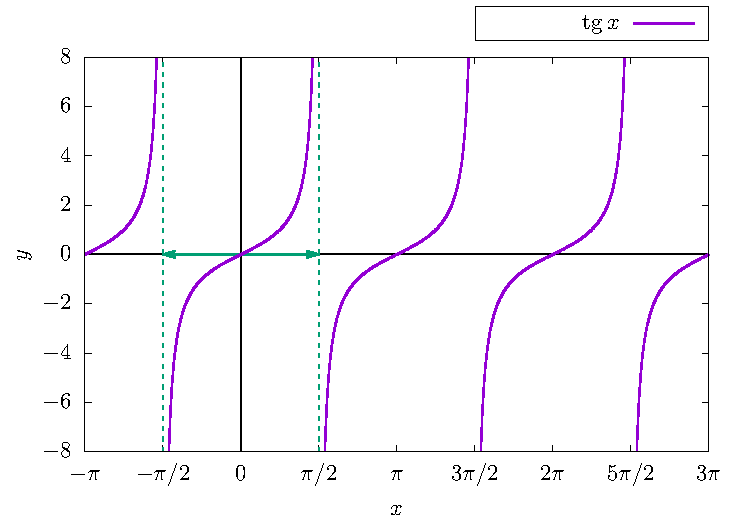
\includegraphics{Gnuplot/cv1/Figures/tangensgraf.pdf}
    \caption{Graf funkce tangens. Zeleně je vyznačen interval, kde je funkce prostá. Ten zvolíme jako obor hodnot funkce arkustangens. Povšimněme si, že v bodech $-\frac{\pi}{2}$ a $\frac{\pi}{2}$ jsou svislé asymptoty. Z nich se stanou vodorovné asymptoty funkce arkustangens.}
    \label{fig:tangens}
\end{figure}

\subsubsection*{Arkuskotangens}

Graf funkce $\cotg x$ je na obrázku \ref{fig:kotangens}. Platí $D(\cotg x) = \R \setminus \set{ k \pi, k \in \mathbb{Z}}$ a $H(\cotg x) = \R$. Interval, na kterém je funkce prostá, je $(0, \pi)$. Definujeme funkci \textbf{arkuskotangens} $\arccotg x$ předpisem 
\begin{align}
    D(\arccotg x) = H(\cotg x) = \R \:, \quad H(\arccotg x) = (0, \pi) \:, \quad \arccotg(x) = y \Longleftrightarrow x = \cotg y \:.
\end{align}

\begin{figure}[H]
    \centering
    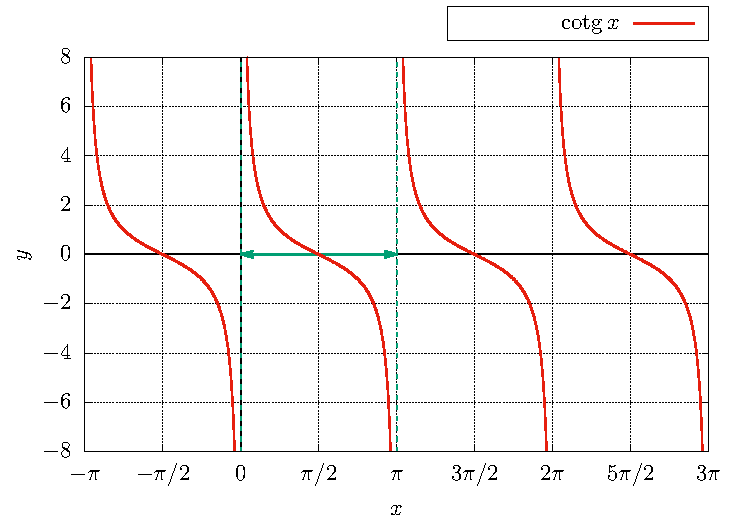
\includegraphics{Gnuplot/cv1/Figures/kotangensgraf.pdf}
    \caption{Graf funkce kotangens. Zeleně je vyznačen interval, kde je funkce prostá. Ten zvolíme jako obor hodnot funkce arkustangens. Povšimněme si, že v bodech $0$ a $\pi$ jsou svislé asymptoty. Z nich se stanou vodorovné asymptoty funkce arkuskotangens.}
    \label{fig:kotangens}
\end{figure}


Grafy funkcí $\arcsin x$ a $\arccos x$ jsou na obrázku \ref{obr:arcsin-arccos}, grafy $\arctg x$ a $\arccotg x$ jsou na obrázku \ref{obr:arctan-arccot}.

\begin{figure}[H]
    \centering
    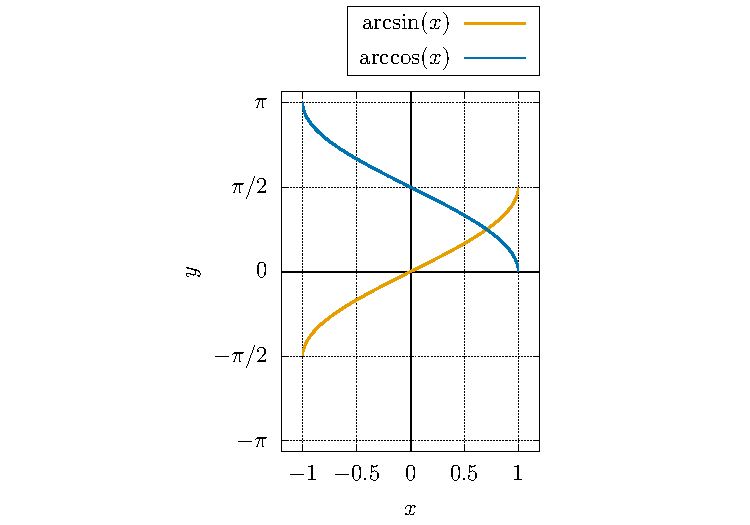
\includegraphics{Gnuplot/cv1/Figures/arcsin-arccos.pdf}
    \caption{Graf funkcí arkussinus a arkuskosinus.}
    \label{obr:arcsin-arccos}
\end{figure}
\begin{figure}[H]
    \centering
    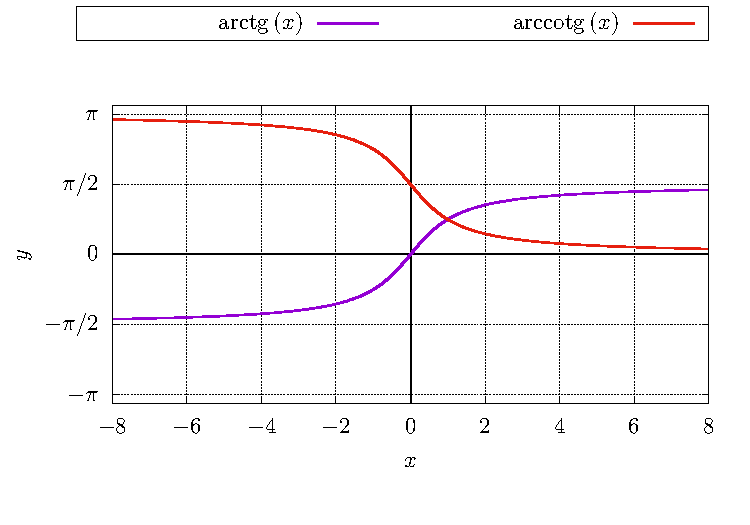
\includegraphics{Gnuplot/cv1/Figures/arctg-arccotg.pdf}
    \caption{Graf funkcí arkustangens a arkuskotangens.}
    \label{obr:arctan-arccot}
\end{figure}
